\section{Motivation}
\subsection{Limitations of address-based scheme}
The current automatic method predicts the lifetime of the data by the address.
That is, AutoStream is based on the assumption that the hotness or lifetime of data 
written to any address space has temporal locality.
In order to see the relationship between the address and the lifetime of data of the append-only workload,
we analyzed the write pattern of RocksDB, one of the popular key-value store.
The lifetime of data is measured by subtracting their logical write time from the invalid time.
Figure~\ref{fig:lba_lifetime} shows the lifetime distribution based on the address and time.
In Figure~\ref{fig:lba_lifetime}(a), all the data have very different lifetimes regardless of their 
address.
However, AutoStream can dynamically adjust the hotness of the address space
according to the access frequency and recency.
If the temporal locality of the hotness is sufficient, 
it is possible to allocate an appropriate stream to the lifetime of the data.
Therefore, we have checked the lifetime of data written in a chunk (1 MB-sized space) over time.
As shown in Figure~\ref{fig:lba_lifetime}(b), it is difficult to allocate the proper stream 
because the lifetime is uneven and the interval with similar lifetime is short.
For append-only workload, it means that the period of enjoying the dynamic allocation is short 
due to the lack of temporal locality of the hotness.
For the automatic stream allocation, thus, more information of the application layer is required.

\begin{figure}[t]
	\centering
	\subfloat[Lifetime by address]{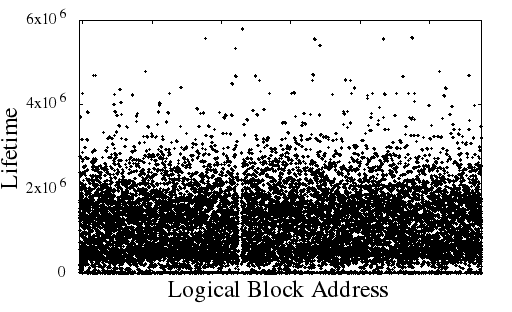
\includegraphics[width=0.25\textwidth]{figure/lba_lifetime}}
	\subfloat[Lifetime by time]{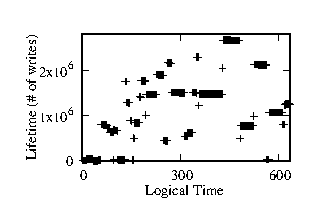
\includegraphics[width=0.22\textwidth]{figure/lifetime_in_chunk}}
	%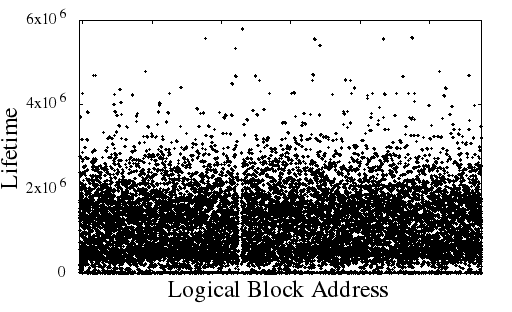
\includegraphics[width=0.9\linewidth]{figure/lba_lifetime} 
	\vspace{-10pt}
	\caption{The lifetime distribution according to the address and time.}
	\label{fig:lba_lifetime}
	\vspace{-15pt}
\end{figure}

%The address-based approach can not properly distinguishes the lifetime of the data written by
%the append-only workload.
%To sum up, although the application knows the lifetime of the written data, it is hard to 
%deliver the information to the system layer without modification.

\subsection{Program context as a lifetime hint}
The lifetime of the data depends on the purpose of the application. 
In general, the writes for different purposes are implemented to have different execution paths.
For example, RocksDB writes a log file and a compaction file in a different functions.

The program context is defined by the summing instruction counter values 
of each execution path of function calls that lead to a write system call which causes write requests,
so it is useful for identifying the purpose of the application. 
Ha et al.~\cite{PCHa} proposed update time based data separator using PC. 
They predicted data update times by exploiting program contexts as hints. 
Since a program context represents a program phase and the same phase is likely to be executed multiple times, 
program contexts have been used in predicting future behavior of programs. 
We extend this approach to differentiate the lifetime of data through invalid time as well as update time. 
In particular, since append-only workloads such as RocksDB have a write-TRIM-write pattern, 
it is necessary to consider an invalid time for an accurate lifetime evaluation.
In previous studies~\cite{MultiStream}, especially for NoSQL DB workload, 
it is known that the lifetime of data can be distinguished by the behavior of applications such as logging, 
flushing, and compaction. 

\begin{figure}[!t]
\centering
\hspace{1pt}
\subfloat[manual: log]{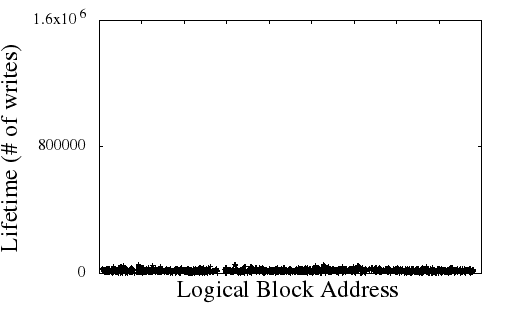
\includegraphics[width=0.23\textwidth]{figure/type_1}}
\subfloat[PC ID: \#2]{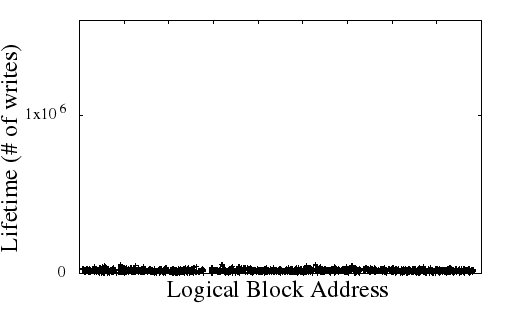
\includegraphics[width=0.23\textwidth]{figure/pcID_2}}
\hfill
\vspace{-10pt}
\subfloat[manual: flush] {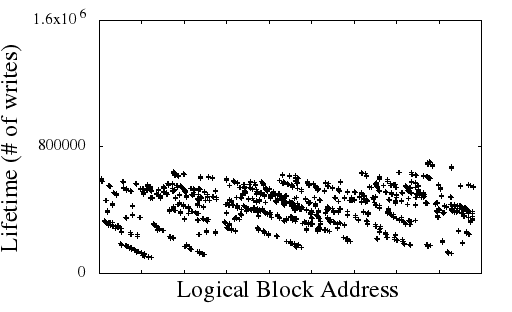
\includegraphics[width=0.23\textwidth]{figure/type_3}}
\subfloat[PC ID: \#3]{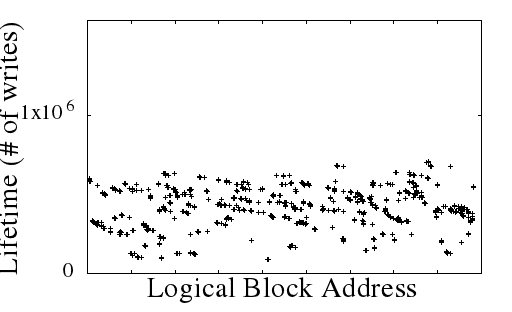
\includegraphics[width=0.23\textwidth]{figure/pcID_3}}
\caption{The lifetime distribution of data types and PCs.} \label{fig:types_and_PCs}
\vspace{-20pt}
\end{figure}

In order to verify that the PC information is enough to recognize the behavior of these applications, 
we ran RocksDB and compared the data lifetimes when the type of data was manually identified 
aginst when the data is identified by PC values.
Figure~\ref{fig:types_and_PCs} shows the lifetime distribution of data separated by manual scheme and 
PC values for two cases, i.e., log and flush.
First, Figure~\ref{fig:types_and_PCs}(a) represents the lifetime of the log file of RocksDB. 
RocksDB's log data is short-lived because the data in memory is temporarily maintained
until the data is flushed to the storage for the consistency reason~\cite{RocksDB}.
Figure~\ref{fig:types_and_PCs}(b) depicts the data lifetime of ID 2 among the classified PCs 
according to the our proposed collection method.
As these two graphs have the same lifetime pattern, we can say PC ID 2 represents the context of the log file.
Similary, Figure~\ref{fig:types_and_PCs}(c) shows the lifetime of flushed static sorted table (SST)
files of RocksDB.
The flush operation stores the memory data as an SST file at level 0 of the LSM tree in the storage.
The file is deleted by a compaction operation that removes invalid data when each level is full.
Due to the characteristics of the LSM tree, which becomes smaller as it goes to top level,
the compaction is often performed at level 0,
so the flushed data at level 0 has a relatively short lifetime~\cite{RocksDB}.
Figure~\ref{fig:types_and_PCs}(d) shows data lifetime of PC ID 3.
As expected, these two graphs have the similar lifetime patterns proving the PC can be a good lifetime hint.


% commentated
\begin{comment}
Recently, various studies are proposed to exploit the stream feature in two .
First, Kang et al.~\cite{MultiStream} proposed that the application
is modified to manually assign streams.
Since an application knows the lifetime of the data best, this approach
is very effective in reducing WAF.
However, in order to properly specify streams in the application, the programmer must
fully understand the lifetime characteristics of the data.
Also when multiple applications try to assign streams, a centralized stream assignment
is required to avoid conflicts.
Second, FStream~\cite{FStream} separates short-lived data, e.g., file system metadata and
journal, using the file system information. 
FStream does not require a burden on the programmer, but the system developer is still burdened
to identify short-lived data of the application, e.g., log data of key-value store, based on the file extension.
In addition, those manual techniques are unable to adapt the stream mapping when the workload or application changes.
These limitations of the manual approach can be overcome by the automatic approach.
Lastly, unlike other schemes, AutoStream~\cite{AutoStream} is aimed to automate the process of mapping 
write I/O operations to an SSD stream.
However, since AutoStream relies on the past LBA access patterns, it is not practical when the data are written in
append-only manner, as modern key-value store.
\end{comment}


